\documentclass[11pt]{article}

\usepackage[margin=1in]{geometry} 
\usepackage{amsmath,amsthm,amssymb,amsfonts}
\usepackage[czech]{babel}
\usepackage[utf8]{inputenc}
\usepackage{enumitem}
\usepackage{ifthen}
\usepackage{tikz}
\usepackage{tikz-qtree}
\usepackage{caption}
%\usepackage{background}
\usepackage{fancyhdr}
\usepackage{picture}
\usepackage{hyperref}

\pagestyle{fancy}
\fancyhf{}
\rhead{Dominika Regéciová, xregec00}
\lhead{PRL 2016/2017, projekt číslo 2}
\rfoot{\thepage}


\begin{document}
% $$
\section{Enumeration sort}
Zadáním projektu bylo implementovat pomocí knihovny Open MPI algoritmus Enumeration sort na lineárním poli o $n$ procesorech dle prezentace do předmětu PRL.\\
Celý program je spouštěn pomocí skriptu s požadovaných počtem prvků: \texttt{./test.sh n}, 
kdy skript vygeneruje soubor s $n$ čísly a spustí kód \textit{es.cpp} s $n+1$ procesory.

\section{Rozbor a analýza algoritmu}
Pro $n$ vstupních prvků je potřeba lineární pole $n$ procesorů doplněnou o společnou sběrnici, schopnou přenést v každém kroku jednu hodnotu.
Každý procesor má stejnou strukturu:\\
$X_i$ -- prvek $x_i$ \\
$Y_i$ -- postupně prvky $x_{1} \dots x_{n}$ \\
$C_i$ -- počet prvků menších než $x_i$ (t.j. kolikrát byl $Y_i \leq X_i$) \\
$Z_i$ -- seřazený prvek $Y_i $\\
Samotný algoritmus má 3 kroky, po kterých máme na výstupu seřazenou posloupnost prvků.\\
1) Všechny registry $C$ se nastaví na hodnotu 1. \\
2) Následující cyklus se opakuje $2n$ krát: \\
2.1) Pokud vstup není vyčerpán, $x_i$ se vloží do $X_i$ (sběrnicí) a do $Y_1$ (lineárním spojením) a obsah všech registrů $Y$ se posune doprava.\\
2.2) Každý procesor s neprázdnými registry $X$ a $Y$ je porovná, a je-li $X > Y$, inkrementuje $C$.\\
2.3) Je-li $k > n$ (t.j. po vyčerpání vstupu) procesor $P_{k-n}$ pošle sběrnicí obsah svého registru $X$ procesoru dle svého registru $C$ ($C$ zde určuje rank cílového procesoru). Cílový procesor si uloží přijatou hodnotu do registru $Z$.\\
3) V $n$ cyklech procesory posouvají obsah svých registrů $Z$ doprava a procesor $P_n$ produkuje seřazenou posloupnost.\\
Takovýto algoritmus není schopen řadit prvky, které obsahují stejné hodnoty. Pro implementaci byla požadovaná modifikace algoritmu pro vyřešení tohoto problému. Změny budou popsány v následující části.\\
Časová složitost je následující:\\
1. krok se provede v konstantním čase $c$\\
2. krok trvá $2n$ cyklů\\
3. krok trvá $n$ cyklů\\
Celkově je tedy časová složitost $t(n) = 3n + c$, což odpovídá lineární složitosti.\\
Počet procesorů $p(n) = n + 1$. \\
Cena $c(n) = p(n) * t(n) = O(n^2)$.\\
Algoritmus není optimální, navíc se výpočet opírá o fakt, že přenos hodnoty přes sběrnici probíhá v konstantním čase.

\section{Implementace}
Program je spouštěn s $n+1$ procesory, kde procesor s rankem $0$ přebírá roli sdílené sběrnice. Jeho úkolem je načtení prvků ze vstupního souboru, distribuce prvků jednotlivým procesorům (s rankem $1$ až $n$) a následně získání výsledků od procesoru $P_n$.
Je to také tento procesor, který vypíše výsledek na výstup.
Kromě hodnot $X$, $Y$, $C$, $Z$ jsou zde boolovské proměnné $nonEmptyX$ a $nonEmptyY$, které značí, zda procesor již má hodnoty X a Y.
Ve své implementaci jsem se snažila co nejvíce držet popsaného algoritmu z prezentací do předmětu PRL.\\
1) 1. krok se provede v podobě přiřazení $1$ do proměnné $C$.\\
2) Počet cyklů zůstává jako v algoritmu, tedy $2n$:\\
2.1) Procesor s rankem $0$ posílá prvky $x_i$, v mém případě však ne od 1. prvku, ale od posledního, jak je naznačeno v příkladu v prezentaci.
Tento prvek přijme procesor $P_1$ do registru $Y$ a procesor $P_k$ do $X$, kde $k$ je čítač cyklů. Také proběhne posun registrů $Y$ doprava.\\
2.2) Pokud jsou hodnoty $nonEmptyX$ i $nonEmptyY$ true, procesor může porovnávat $X$ a $Y$. Právě zde nastává změna od původního algoritmu.
Změna je inspirována materiálem:\\ \url{http://citeseerx.ist.psu.edu/viewdoc/download?doi=10.1.1.106.4976&rep=rep1&type=pdf}.
Každý procesor porovnává $X$ a $Y$ dvěma způsoby -- $X > Y$ nebo $X \geq Y$, záleží na pozici prvku v porovnání s rankem procesoru.
Například procesor $P_3$ porovnává na $X \geq Y$ první $3$ prvky, zbylé porovnává na $X > Y$.\\
2.3) Po vyčerpání vstupu a dokončení porovnání vždy jeden procesor rozešle informaci, že bude posílat $X$ procesoru s rankem $C$. Ten přijme hodnotu a uloží si ji do registru $Z$.\\
3) Poslední krok se provede $n$ krát -- procesor $P_n$ zašle $P_0$ výsledné Z, které $P_0$ vloží do výstupního pole (vkládá od konce, aby vznikla
seřazená posloupnost od nejmenší po největší prvek). Pak dojde k posunu Z hodnot doprava.

\section{Testování}
Testování jsem spouštěla přes automatizované testy.
Nejdříve jsem testovala správnost implementace algoritmu a maximální počet prvků pro nastavení na merlinovi. Zde se limitem stalo $25$ procesorů.
Poté jsem tedy testovala v rozsahu $1$ až $25$ procesorů (včetně), přičemž každý rozsah jsem testovala $10$ krát. 
Testy jsem spustila celkově $3$ krát.
Časové hodnoty jsou zprůměrované -- nejdřív průměr $10$ testů a pak průměr $3$ vzniklých hodnot na $n_i$ počet prvků. I tak jsou však místy viditelné odchylky způsobené operačním systémem.

\begin{figure}[h]
\centering
\includegraphics[scale=0.5]{graf.eps}
\caption{Graf výsledků testování}
\end{figure}

\newpage
\section{Komunikační protokol}
\begin{figure}[h]
\centering
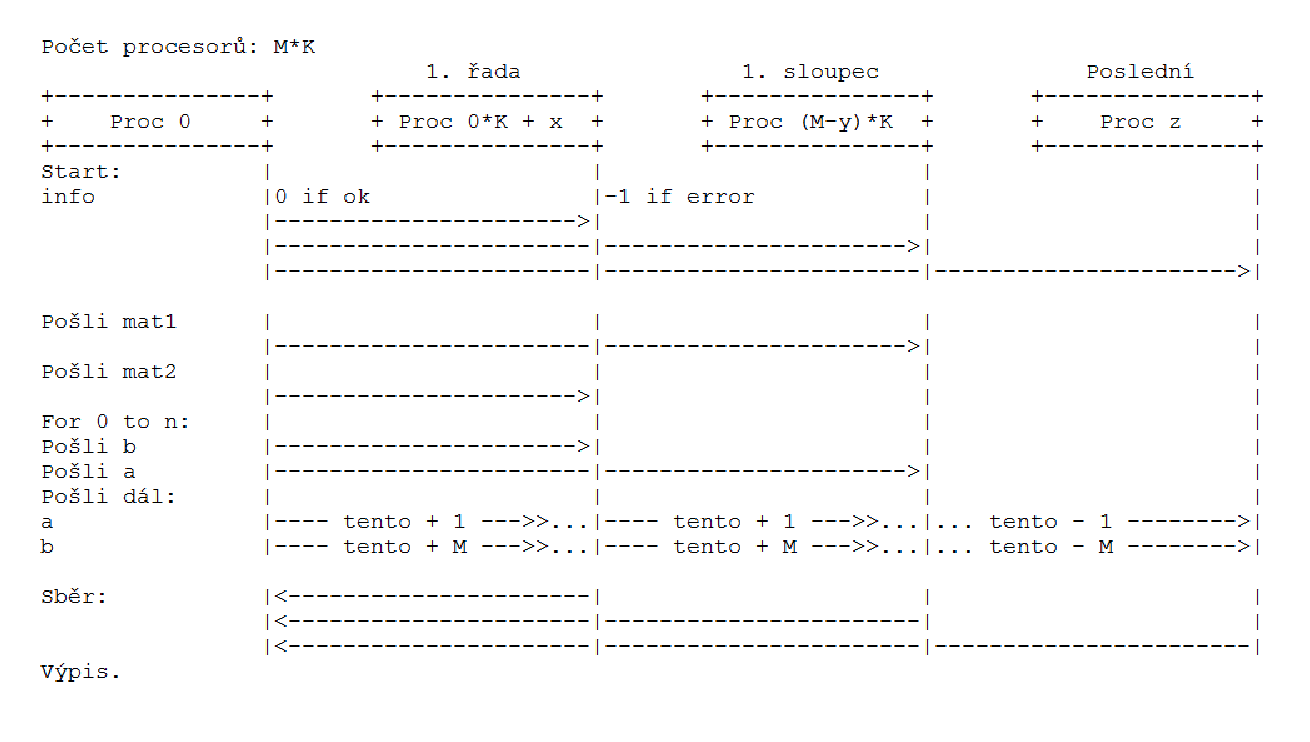
\includegraphics[scale=0.7]{diagram.eps}
\caption{Sekvenční diagram pro n procesorů}
\end{figure}

\section{Závěr}
Seznámila jsem se s knihovnou Open MPI pro programování paralelních výpočtů a úspěšně jsem implementovala Enumeration sort na lineárním poli o n procesorech dle prezentace do předmětu PRL.
Podařilo se mi zavést úpravu implementace, aby algoritmus dokázal řadit i posloupnost prvků s vícero výskyty stejných prvků.
Analýza i testování pak ukázaly, že algoritmus pracuje v lineárním čase.

\end{document}
